


%\begin{document}

%Portada del Documento
\chapter{HasKell}
\setlength{\unitlength}{0.5 cm} %Especificar unidad de trabajo
\thispagestyle{empty}
\begin{picture}(18,12)
\put(2,0){
\includegraphics[width=12cm,height=5cm]{./imagenes5/logo.png}}
\end{picture}



% fin de la portada


\newpage
\section{ Introducción}

Mastermind (Español "Mente maestra") es un juego de mesa, de ingenio y reflexión, para dos jugadores.
Se juega en un tablero con fichas blancas y negras pequeñas y de otros colores, de un tamaño algo superior. Uno de los jugadores escoge un número de fichas de colores, 4 en el juego original, y pone un código secreto oculto del otro jugador. Éste, tomando fichas de colores del mismo conjunto, aventura una posibilidad contestada con negras (fichas de color bien colocadas) o blancas (fichas de color con el color correcto, pero mal colocadas).
Termina al averiguarse la combinación (es decir, se consigue una combinación con cuatro negras), o bien se agota el tablero (depende del tamaño, aunque generalmente son 15 combinaciones).
Mastermind es actualmente una marca comercial propiedad de Pressman Toys; el origen puede derivar de un juego tradicional inglés denominado Toros y vacas, se jugaba sobre papel: los "toros" equivalían a las fichas negras, y las "vacas" a las blancas.

\section{ Descripción del Algoritmo Genético}
nuestro algoritmo se baso en el paper:
 \url {http://www.cs.bris.ac.uk/Publications/Papers/2000067.pdf}
\begin{enumerate}[1)]
 \item Pedir el pool y la longitud de la conjetura por teclado.
 \item Generar la primera conjetura aleatoriamente de acuerdo a la longitud ingresada
 \item setear el cfg
 \item  Mostrar al usuario la conjetura
  \item  Pedir al usuario que califique la conjetura
 \item recibir el resultado de blancas y negras por parte del usuario  
 \item Determinar si el cfg debe ser cambiado por la conjetura actual de acuerdo a los siguientes parametros:
         \begin{enumerate}[a)]
         \item Si las blancas de la conjetura actual es mayor a las  blancas del cfg entonces. Cambio cfg
         \item Si las blancas de la conjetura actual son igual a las  blancas del cfg, Si las negras de la conjetura actual son mayor a las  negras del cfg entonces Cambio cfg
    \end{enumerate}
 \item Segun la cantidad de negras y blancas del cfg hacer una de las siguientes opciones:
          \begin{enumerate}[a)]
         \item Si las blancas son igual en longitud de la conjetura y las negra son igual a cero entonces ha ganado el juego
         \item Si las blancas son igual a cero y las negras son igual a cero entonces elimina las letras del pool, anade las letras a la lista de posiciones imposibles(puede ser opcional) y genera una nueva conjetura inicial
         \item Si las blancas son igual a cero y las negras son diferentes de cero entonces añade las letras a la lista de posiciones imposibles
         \item Si las blancas mas las negras son igual en longitud a la conjetura y las negras son diferentes de cero y las blancas son diferentes de cero entonces el pool solo se queda con dichas letras
    \end{enumerate}
 \item Generar una nueva congetura siguiendo los siguientes parametros
             \begin{itemize}
              \item Por cada elemento que no haya estado en correcta posicion(longitud del cfg - blancas)
                       \begin{itemize}
                           \item Escoger una letra del cfg al azar
                            \item Escoger una letra del pool al azar
                            \item Reemplazar letra de la conjetura por la letra del pool(en la misma ubicacion que estaba la letra de la conjetura)
                        \end{itemize}
              \end{itemize}
 \item Chequear la conjetura generada en la lista de imposibles de acuerdo al lo siguiente
            \begin{itemize}
              \item Si alguna letra de la nueva conjetura esta en la lista de imposibles
               \item regreso al paso 10
              \end{itemize}
 \item Repetir desde el paso 4 hasta que se acabe el juego o hasta que el usuario haya tenido 10 intentos 

\end{enumerate}
  
\section{ El proyecto}

  \subsection{ Requisitos}

Se necesita tener instalado el compilador para el lenguaje Haskell , este se lo puede encontrar en las pagina oficial del lenguaje:
 \url{  http://www.haskell.org}
\begin{figure}[htb]
\centering
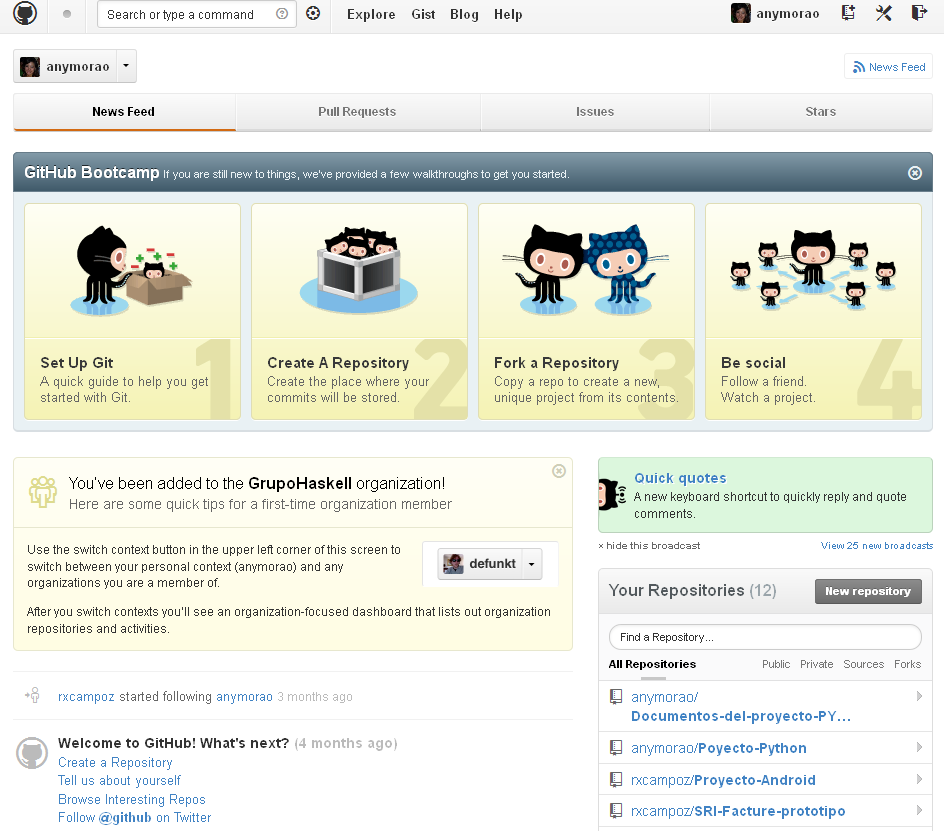
\includegraphics[width=0.57\textwidth]{./imagenes5/Dibujo1.png}
\end{figure}

 \subsection{ Como Ejecutar el Proyecto}
\begin{enumerate}[a)]
     \item Abrimos el WinGHCi 
     \item Cargamos Base2.hs
    \item Cargamos Controlador2.hs
    \item Cargamos Principal2.hs
    \item Evaluamos
\end{enumerate}

\begin{figure}[ht!]

   \centering     %%----primera subfigura----
   \subfloat[]{
        \label{fig:pantalla:1}         %% Etiqueta para la primera subfigura
        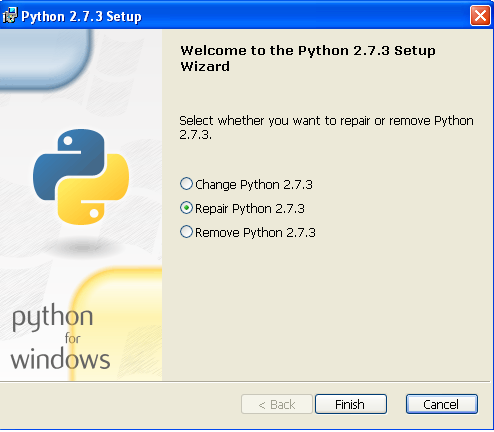
\includegraphics[width=0.42\textwidth]{./imagenes5/img2.png}}
   \hspace{0.1\linewidth}
   %%----segunda subfigura----
   \subfloat[]{
        \label{fig:pantalla:2}         %% Etiqueta para la segunda subfigura
        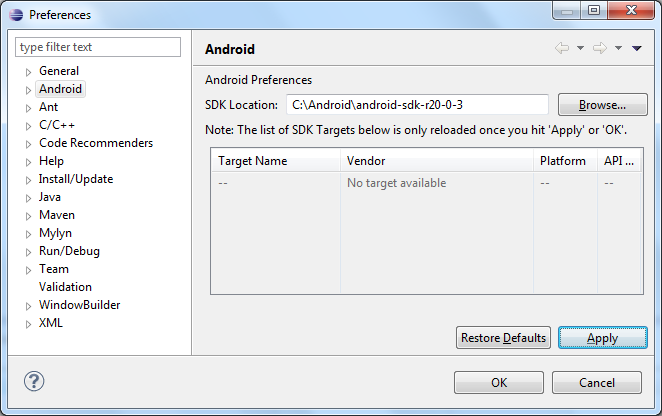
\includegraphics[width=0.42\textwidth]{./imagenes5/img3.png}}\\[20pt]
   %%----tercera subfigura----
   \subfloat[]{
        \label{fig:pantalla:3}         %% Etiqueta para la tercera subfigura
        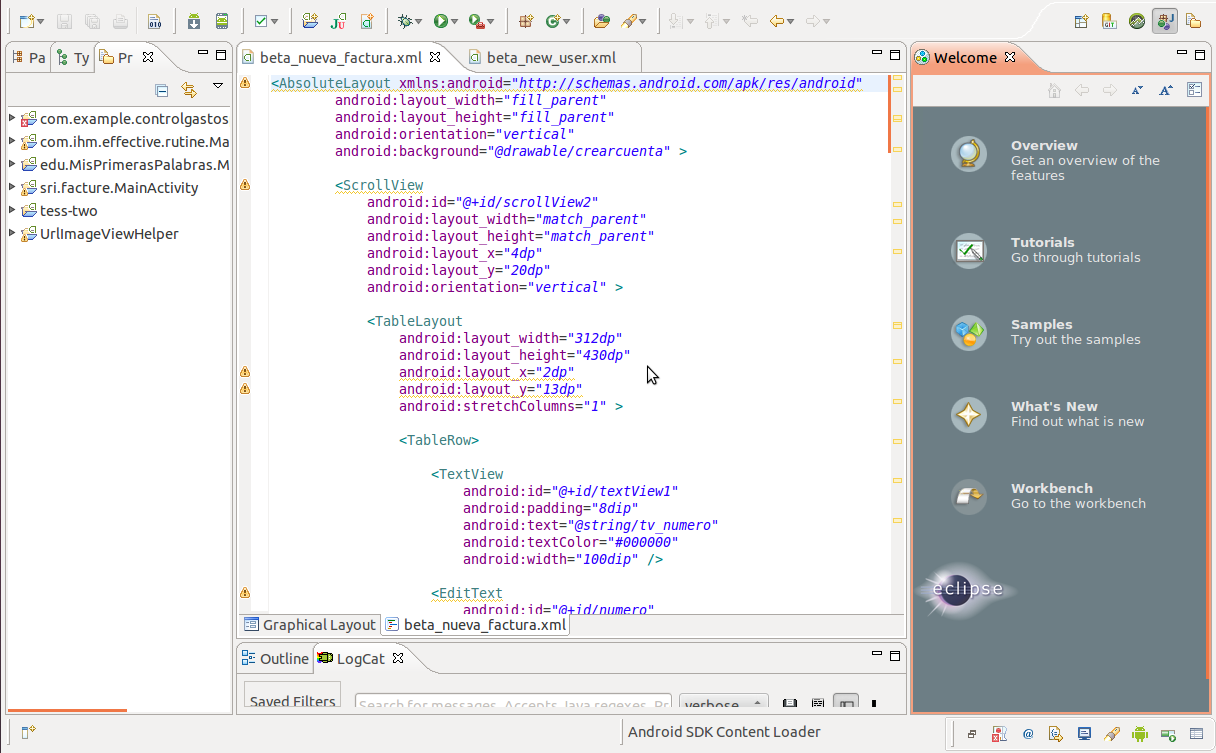
\includegraphics[width=0.42\textwidth]{./imagenes5/img4.png}}
    
   %%----cuarta subfigura----
    \subfloat[]{
        \label{fig:pantalla:4}         %% Etiqueta para la cuarta subfigura
        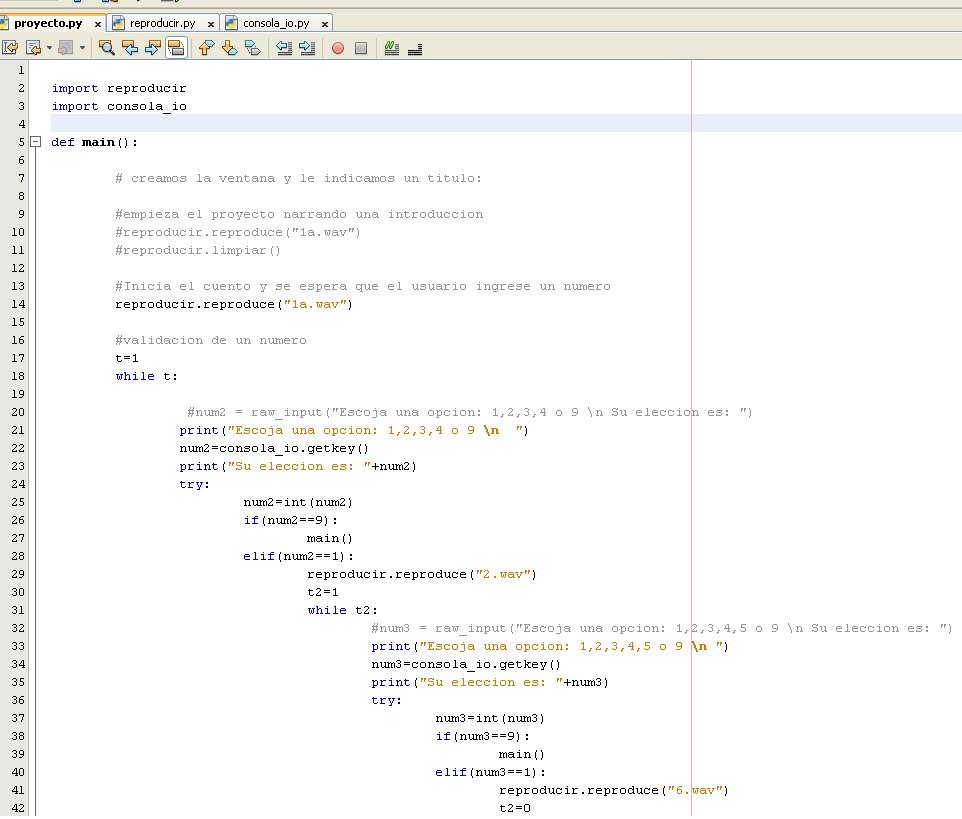
\includegraphics[width=0.42\textwidth]{./imagenes5/img5.png}}
\hspace{0.1\linewidth}
%%----Quinta subfigura----
    \subfloat[]{
        \label{fig:pantalla:5}         %% Etiqueta para la quintasubfigura
        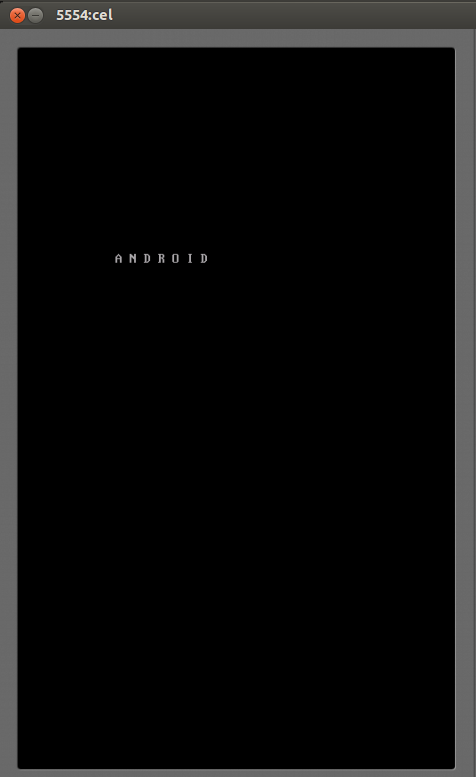
\includegraphics[width=0.42\textwidth]{./imagenes5/img6.png}}


\end{figure}

\subsubsection{Inicio del Mastermind}
 \begin{itemize}
   \item  Despues de cargar todos los archivos y de evaluar el programa me pide que ingrese el pool de letras (en este caso se ingreso abcde), las cuales pueden ser maximo 10 letras una vez ingresado el pool doy enter e inmediatamente me pide que ingrese la longitud del codigo a descifrar (en este caso el codigo a desifrar tiene longitud 4).
        \begin{figure}[htb]
        \centering
        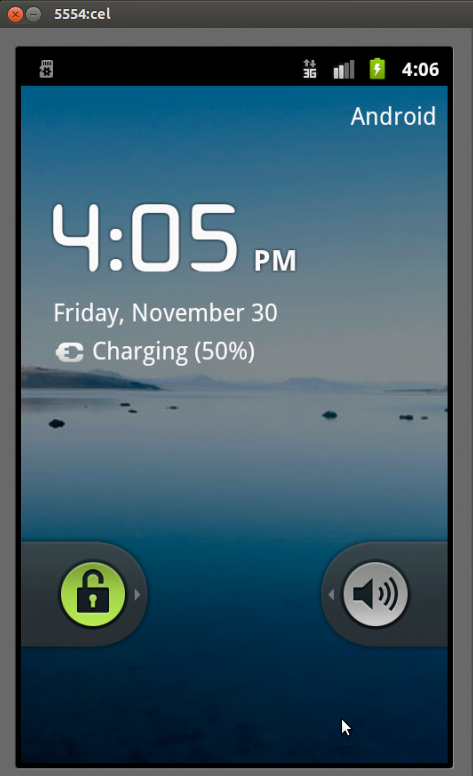
\includegraphics[width=0.99\textwidth]{./imagenes5/img7.png}
        \end{figure}

  \item A continuación me genera una conjetura la cual tengo que evaluar poniendo :
          \begin{itemize}
          \item El número de letras en posición correcta
          \item El número de letras en posición incorrecta
          \end{itemize}
  En este caso no hay ninguna letra en posición correcta pero si estan las 4 letras que pertenecen al codigo que debe adivinar.
 \begin{figure}[htb]
        \centering
        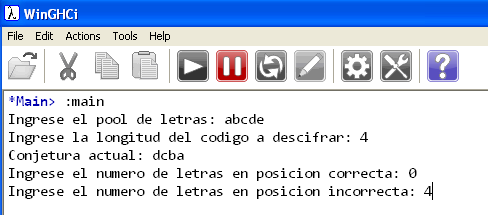
\includegraphics[width=0.99\textwidth]{./imagenes5/img8.png}
        \end{figure}
\item cuando el número de letras en la posición correcta en igual a la longitud a descifrar y l las letras en posicion corecta es 0 entonces sale un mensaje de felicitaciones ganaste.
        \begin{figure}[htb]
        \centering
        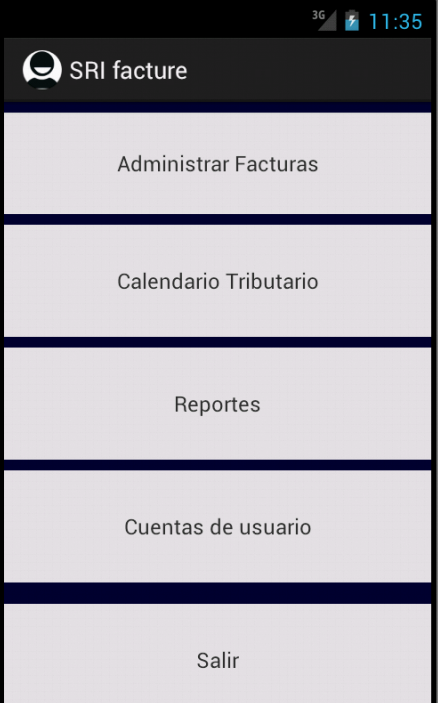
\includegraphics[width=0.99\textwidth]{./imagenes5/img9.png}
        \end{figure}

 \end{itemize}

\section{Programa Fuente}

 \begin{itemize}
      \item BASE

        \begin{verbatim}
           module Base2
           ( Conjetura (..)
           , Imposibles (..)
           , conjetura_codigo
           , conjetura_aciertos
           , conjetura_errores
            , imposible_letra
            , imposible_pos
            ) where
        {------------------------------------------------------}
           data Conjetura = Conjetura String Int Int
                 deriving(Show)
         conjetura_codigo(Conjetura codigo _ _) = codigo

          conjetura_aciertos(Conjetura _ aciertos _) = aciertos

          conjetura_errores(Conjetura _ _ errores) = errores 

          data Imposibles = Imposibles Char Int
                deriving(Show)

       imposible_letra(Imposibles letra _) = letra
       imposible_pos(Imposibles _ posicion) = posicion

     {---------------------------------------------------------}
      \end{verbatim}
          \item CONTROLADOR

                \begin{verbatim}
              import Controlador2
import Base2

{---------------------------------------------------------------------------------------}

nameLambda (contador , cfg, codigo , tam , pool , imposibles , historial , bln) =
         if (codigo == "trampa-") then
             putStr "Tramposo, has dado una mala retroalimentacion, el pool esta vacio\n\n Tu historial ha sido: " >>
             putStr historial >>
              putStr "\n"
          else
              if (contador == 10) then
                   putStr "Perdiste, agotaste tus 10 intentos\n\n  Tu historial ha sido: " >>
                   putStr historial >>
                   putStr "\n"
              else
                    if (bln == tam) then
                        putStr "Felicitaciones , ganaste\n\n Tu historial ha sido: " >>
                        putStr historial >>
                        putStr "\n"
                    else
                        if (contador == 1 ) then
			        putStr "Ingrese el pool de letras: " >>
			        getLine >>=
			        \first -> putStr "Ingrese la longitud del codigo a descifrar: " >>
			        getLine >>=
			        \last -> let pool_inicio = first
				           longitud = stringtoInt (last)
		                            codigo_inicio = conjetura_inicial (pool_inicio , longitud , [] , 1 )
		                             cont_aux = contador + 1
		                             cfg_inicial = Conjetura codigo_inicio 0 0
		                             in nameLambda (cont_aux , cfg_inicial , codigo_inicio , longitud , pool_inicio , imposibles , historial , bln)
		                             
		       else
                                putStr "Conjetura actual: " >>
                                 putStr codigo >>
		               putStr "\nIngrese el numero de letras en posicion correcta: " >>
			       getLine >>=
			        \blancas -> putStr "Ingrese el numero de letras en posicion incorrecta: " >>
			        getLine >>=
			        \negras -> let historial_new = cambia_historial (codigo , historial)
                                               aciertos = stringtoInt (blancas)
				              errores = stringtoInt (negras)
		                               conjetura = Conjetura codigo aciertos errores
		                               cfg_new = cambiar_cfg (cfg , conjetura)
		                               imposibles_new = cambiar_imposibles (imposibles , cfg_new)
		                               ( pool_new , bandera ) = cambiar_pool (cfg_new , pool , tam)
		                               conjetura_gen = crear_conjetura (cfg_new , pool_new , imposibles , 1 , bandera)
		                             cont_new = contador + 1
				      in  nameLambda (cont_new , cfg_new , conjetura_gen , tam , pool_new , imposibles_new , historial_new , aciertos)


{------------------------------------------------------------------------------------------------------------------------------------------}      
   
main = nameLambda ( 1 , Conjetura "ggg" 0 0 , "ggggg" , 4 , "abcdef" , [] , " " , 0 )

                \end{verbatim}

       \item PRINCIPAL

                  \begin{verbatim}
                 module Controlador2
( cambiar_cfg
, nuevo_imposible
, cambiar_imposibles
, elimina_letras_pool
, cambiar_pool
, valida_posicion
, ubica_letra
, crear_conjetura
, stringtoInt
, cambia_historial
, imprimir_conjetura
, imprimir_historial
, conjetura_inicial
, inttoString
) where

import Base2


{----------------------------------------------------------------------------------------------------------------------}
cambiar_cfg (conjetura , cfg) = 
         let
            aciertos_cfg = conjetura_aciertos (cfg)
            aciertos_conj = conjetura_aciertos (conjetura)
            errores_cfg = conjetura_errores (cfg)
            errores_conj = conjetura_errores (conjetura)
         in
            if ( (aciertos_conj > aciertos_cfg) || (aciertos_cfg == aciertos_conj && errores_conj > errores_cfg) ) then
               conjetura
            else
               cfg

{------------------------------------------------------------------------------------------------------------------------}

nuevo_imposible ( [] , imposible , posicion ) = imposible {---ojo con el []--}
nuevo_imposible ( cadena , imposible , posicion ) = 
         let
            letra = head (cadena)
            imp = Imposibles letra  posicion
            conc = imp : imposible
            cola = tail (cadena)
            pos_new = posicion + 1
         in
            nuevo_imposible (cola , conc , pos_new)


{---------------------------------------------------------------------------------------------------------------------------}

cambiar_imposibles (imposibles , cfg) = 
         let
           aciertos = conjetura_aciertos (cfg)
           errores = conjetura_errores (cfg)
           aux = conjetura_codigo (cfg)
           cont = 1
         in
           if (aciertos == 0 && errores /= 0 ) then
              nuevo_imposible (aux , imposibles , cont)
           else
              imposibles


{----------------------------------------------------------------------------------------------------------------------------}

elimina_letras_pool (codigo , [] , arreglo) = arreglo
elimina_letras_pool (codigo , pool , arreglo) = 
         let
           ele = head (pool)
           col = tail (pool)
           band = ele `elem` codigo
           conc = ele : arreglo
         in
           if (band == False ) then
              elimina_letras_pool (codigo , col , conc)
           else
              elimina_letras_pool (codigo , col , arreglo)
           
{-----------------------------------------------------------------------------------------------------------------------------}

cambiar_pool (cfg , pool , longitud) =
         let
           aciertos = conjetura_aciertos (cfg)
           errores = conjetura_errores (cfg)
           codigo = conjetura_codigo (cfg)
         in
           if (aciertos == 0 && errores == 0) then
              ( elimina_letras_pool (codigo , pool , [] ) , False )
           else
              if (aciertos + errores == longitud) then
                 ( codigo , True )
              else
                 ( pool , True )


{-------------------------------------------------------------------------------------------------------------------------------}

valida_posicion (letra_pool , num_cod , [] ) = True
valida_posicion (letra_pool , num_cod , imposibles) = 
         let
           imp = head (imposibles)
           letra = imposible_letra (imp)
           pos = imposible_pos (imp)
         in
           if (letra == letra_pool && pos == num_cod) then
              False
           else
              valida_posicion (letra_pool , num_cod , tail (imposibles) )

{-------------------------------------------------------------------------------------------------------------------------------}  

ubica_letra (codigo , letra_pool , num_cod) =
        let
          ( x , y ) = splitAt num_cod codigo
          aux = letra_pool : y
        in
          init (x) ++ aux

{----------------------------------------------------------------------------------------------------------------------------------}

crear_conjetura (cfg , pool , imposibles , cont , bandera) = 
       let
         aciertos = conjetura_aciertos (cfg)
         errores = conjetura_errores (cfg)
         codigo = conjetura_codigo (cfg)
         long_cod = length (codigo)
         long_pool = length (pool)
         num_cod = 3 {-numero_aleatorio (1 , long_cod)-}
         num_pool = 3 {-numero_aleatorio (1 , long_pool)-}
         letra_cod = codigo !! (num_cod - 1)
         letra_pool = pool !! (num_pool - 1)
         aux = long_cod - aciertos
         letra_ok = ubica_letra (codigo , letra_pool , num_cod)
         cfg_new = Conjetura letra_ok aciertos errores 
         cont_new = cont + 1
      in
         if ( null (pool) == True ) then
            "trampa-"
         else   
            if ( bandera == False ) then
               conjetura_inicial (pool , long_cod , [] , 1 )
            else
               if ( valida_posicion ( letra_pool , num_cod , imposibles) == False ) then
                  crear_conjetura (cfg , pool , imposibles , cont , bandera)
               else
                  if (cont >= aux) then
                     letra_ok
                  else
                     crear_conjetura (cfg_new , pool , imposibles , cont_new , bandera)
   
               
{--------------------------------------------------------------------------------------------------------------------}


stringtoInt (cad) = 
      if (cad == "0") then 0 else if (cad == "1") then 1 else if (cad == "2") then 2 else if (cad == "3") then 3 else if (cad == "4") then 4 else if (cad == "5") then 5 else if (cad == "6") then 6 else if (cad == "7") then 7 else if (cad == "8") then 8 else if (cad == "9") then 9 else if (cad == "10") then 10 else 20

{-----------------------------------------------------------------------------------------------------------------------}

{-pedir_retroalimentacion (conjetura) = 
      do
        putStrLn "Escriba el numero de letras en correcta posicion: \n"
        s <- getLine
        putStrLn "Escriba el numero de letras en incorrecta posicion: \n"
        x <- getLine
        let
           aciertos = stringtoInt (s)
           errores = stringtoInt (x)
           conj_new = Conjetura conjetura aciertos errores 
        return conj_new-}

{------------------------------------------------------------------------------------------------------------------------}

cambia_historial (conjetura , historial) = conjetura ++ "-------" ++ historial 

{------------------------------------------------------------------------------------------------------------------------}

imprimir_conjetura (conjetura) = putStrLn $ "-------------------Conjetura actual: "++conjetura++" ---------------------"

{------------------------------------------------------------------------------------------------------------------------}

imprimir_historial (historial) = putStrLn $ "------------------- "++historial++"---------------------"

{--------------------------------------------------------------------------------------------------------------------------}

conjetura_inicial ([] , longitud , arreglo , contador) = conjetura_inicial ( tail (arreglo) , longitud , arreglo , contador)
conjetura_inicial (pool , longitud , arreglo , contador) = 
        let
           aux = head (pool)
           conc = aux : arreglo
           cont = contador + 1
           col = tail (pool)
        in
          if (longitud == contador) then
             conc
          else
             conjetura_inicial ( col , longitud , conc , cont)
         
{---------------------------------------------------------------------------------------------}

inttoString (cad) =
        if (cad == 0) then "0" else if (cad == 1) then "1" else if (cad == 2) then "2" else if (cad == 3) then "3" else if (cad == 4) then "4" else if (cad == 5) then "5" else if (cad == 6) then "6" else if (cad == 7) then "7" else if (cad == 8) then "8" else if (cad == 9) then "9" else if (cad == 10) then "10" else "20"


     \end{verbatim}

  \end{itemize}

\section{Experiencias}
\begin{itemize}
\item Haskell fue un lenguaje dificil de entender para mi debido a lo complicado de la programacion funcional.
\item Haskell no tiene mucha funcionalidades como las tienen lo demas lenguajes de programación secuenciales.
\item Tuve muchos problemas en realizar la parte del proyecto q me tocaba ya que no encontraba como generar de forma aleatoria la conjetura.
\item Tambien tuvimos problemas con uno de mis compañeros de grupo, que no trabajo su parte del proyecto.
\item La parte de aleatoriedad en la que teniamos problemas, pudimos resolverla a último minuto pero aun tiene fallas al generar la conjetura.
 \end{itemize}

%\end {document}

